% Previous horizontal figure preserved for review:
% % Figure 2(b): final 1 TB single-run measurements. The 1 KB Conventional cell
% % is from figure2_1tb_fourcell_260903_run1; the other three cells are from
% % figure2_1tb_fourcell_260903_resume1. WAF uses profiler-attributable SST bytes.
% \begin{tikzpicture}[
%     x=1cm,
%     y=1cm,
%     font=\normalsize,
%     axis/.style={draw=black!75, line width=0.45pt},
%     flushOnly/.style={draw=blue!75!black, fill=blue!30, dashed},
%     conventional/.style={draw=blue!75!black, fill=blue!70, dashed}
% ]
% \path[use as bounding box] (-0.30,-0.05) rectangle (5.45,4.80);
% \draw[axis] (0.75,0.95) -- (5.35,0.95);
% \draw[axis] (0.75,0.95) -- (0.75,4.15);
% 
% % Linear scale: 0--5 hours over 3.2 cm.
% \foreach \y/\label in {0.950/0,1.590/1,2.230/2,2.870/3,3.510/4,4.150/5} {
%     \draw[black!12, line width=0.35pt] (0.75,\y) -- (5.35,\y);
%     \draw[axis] (0.70,\y) -- (0.75,\y);
%     \node[anchor=east, font=\normalsize] at (0.64,\y) {\label};
% }
% 
% % 1 KB: Flush-only 1,327 s (WAF 1.016459),
% % Conventional 3,840 s (WAF 12.777716).
% \draw[flushOnly]   (1.55,0.95) rectangle (2.05,1.185911);
% \draw[conventional](2.05,0.95) rectangle (2.55,1.632667);
% \node[anchor=west, rotate=90, font=\normalsize] at (1.80,1.24) {1.02$\times$};
% \node[anchor=west, rotate=90, font=\normalsize] at (2.30,1.69) {12.78$\times$};
% \node[anchor=north, font=\normalsize] at (2.05,0.88) {1KB};
% 
% % 91 B: Flush-only 10,119 s (WAF 1.086737),
% % Conventional 13,754 s (WAF 15.292634).
% \draw[flushOnly]   (3.55,0.95) rectangle (4.05,2.748933);
% \draw[conventional](4.05,0.95) rectangle (4.55,3.395156);
% \node[anchor=west, rotate=90, font=\normalsize] at (3.80,2.81) {1.09$\times$};
% \node[anchor=west, rotate=90, font=\normalsize] at (4.30,3.46) {15.29$\times$};
% \node[anchor=north, font=\normalsize] at (4.05,0.88) {91B};
% 
% \node[rotate=90, anchor=south, font=\Large] at (-0.02,2.55)
%     {Loading time (hours)};
% \node[anchor=north, font=\normalsize] at (3.05,0.43) {KV size (1 TB)};
% \draw[flushOnly] (0.90,4.34) rectangle (1.22,4.58);
% \node[anchor=west, font=\normalsize] at (1.32,4.46) {Flush-only};
% \draw[conventional] (3.15,4.34) rectangle (3.47,4.58);
% \node[anchor=west, font=\normalsize] at (3.57,4.46) {Conventional};
% \end{tikzpicture}

% Active vertical figure generated from the promoted TSV data.
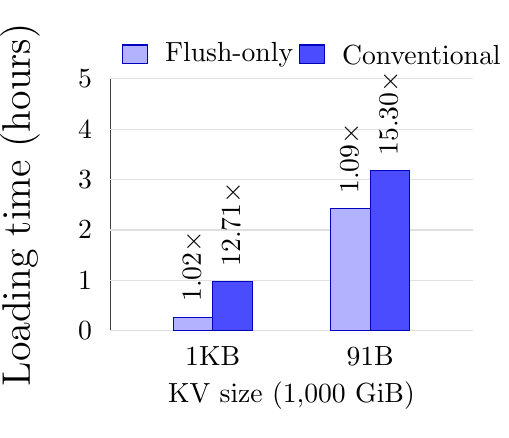
\begin{tikzpicture}[x=1cm,y=1cm,font=\normalsize,
axis/.style={draw=black!75,line width=0.45pt},
flushOnly/.style={draw=blue!75!black,fill=blue!30},
conventional/.style={draw=blue!75!black,fill=blue!70}]
\path[use as bounding box] (-0.30,-0.05) rectangle (5.45,4.80);
\draw[axis] (0.75,0.95)--(5.35,0.95);
\draw[axis] (0.75,0.95)--(0.75,4.15);
\draw[black!12] (0.75,0.95000)--(5.35,0.95000);
\node[anchor=east] at (0.64,0.95000) {0};
\draw[black!12] (0.75,1.59000)--(5.35,1.59000);
\node[anchor=east] at (0.64,1.59000) {1};
\draw[black!12] (0.75,2.23000)--(5.35,2.23000);
\node[anchor=east] at (0.64,2.23000) {2};
\draw[black!12] (0.75,2.87000)--(5.35,2.87000);
\node[anchor=east] at (0.64,2.87000) {3};
\draw[black!12] (0.75,3.51000)--(5.35,3.51000);
\node[anchor=east] at (0.64,3.51000) {4};
\draw[black!12] (0.75,4.15000)--(5.35,4.15000);
\node[anchor=east] at (0.64,4.15000) {5};
% flush_only_1kb: 979.726168394 s, WAF 1.016491424, source /home/smrc/virtual_compaction/vcomp/experiments/artifacts/log_loads/paper_ch23_common_260905_approved_run3/full/flush_only_1kb
\draw[flushOnly] (1.5500,0.95) rectangle (2.0500,1.12417);
\node[anchor=west,rotate=90] at (1.8000,1.19417) {1.02$\times$};
% baseline_1kb: 3501.417249680 s, WAF 12.713699587, source /home/smrc/virtual_compaction/vcomp/experiments/artifacts/log_loads/paper_ch23_common_260905_approved_run3/full/baseline_1kb
\draw[conventional] (2.0500,0.95) rectangle (2.5500,1.57247);
\node[anchor=west,rotate=90] at (2.3000,1.64247) {12.71$\times$};
\node[anchor=north] at (2.0500,0.88) {1KB};
% flush_only_91b: 8711.426300049 s, WAF 1.086763494, source /home/smrc/virtual_compaction/vcomp/experiments/artifacts/log_loads/paper_ch23_common_260905_approved_run3/full/flush_only_91b
\draw[flushOnly] (3.5500,0.95) rectangle (4.0500,2.49870);
\node[anchor=west,rotate=90] at (3.8000,2.56870) {1.09$\times$};
% baseline_91b: 11426.155120373 s, WAF 15.303675270, source /home/smrc/virtual_compaction/vcomp/experiments/artifacts/log_loads/paper_ch23_common_260905_approved_run3/full/baseline_91b
\draw[conventional] (4.0500,0.95) rectangle (4.5500,2.98132);
\node[anchor=west,rotate=90] at (4.3000,3.05132) {15.30$\times$};
\node[anchor=north] at (4.0500,0.88) {91B};
\node[rotate=90,anchor=south,font=\Large] at (-0.02,2.55) {Loading time (hours)};
\node[anchor=north] at (3.05,0.43) {KV size (1,000 GiB)};
\draw[flushOnly] (0.90,4.34) rectangle (1.22,4.58);
\node[anchor=west] at (1.32,4.46) {Flush-only};
\draw[conventional] (3.15,4.34) rectangle (3.47,4.58);
\node[anchor=west] at (3.57,4.46) {Conventional};
\end{tikzpicture}
